\documentclass[
    alternativetitlepage=alternativ,
    cornerlogo=hgi_nds_logo2,
    sectionoverview,
]{rubpresentation}
\setbeamercovered{invisible}

\title[XML/JSON conversions]
{Bridging the Gap: Secure and lossless conversion\\ of XML data structures to the JSON format}
\subtitle{\small Bachelor thesis \hspace{3mm}{\scriptsize $\blacksquare$}\hspace{3mm} March 30, 2017 -- June 29, 2017}

\author[Holthuis]{Jan~Holthuis}

\institute[Advisors]
{%\inst{1}%
Advisors: Dennis Felsch \& Paul Rösler
}
\date{July 4, 2017}
\subject{Computer Science}

\titlegraphic{datacenter.jpg}
\sponsorlogo[height=7.6mm,interpolate=true]{hgi_nds_logo}

\definecolor{rubblue}{HTML}{003660}
\definecolor{rubgreen}{HTML}{8dae10}
\definecolor{rubgray}{HTML}{e7e7e7}

\usepackage{minted}
\usemintedstyle{rub}

\usepackage{mathtools}
\usepackage{tikzsymbols}
\setbeamercovered{invisible}

\AtBeginSubsection[]{%
  \begin{frame}%
    \frametitle{\iflanguage{english}{Overview}{Überblick}}%
    \tableofcontents[currentsubsection]%
  \end{frame}%
}%

\begin{document}

\frame[plain]{\titlepage}

%\begin{frame}{The \texttt{\textbackslash note}-Macro}
%\begin{itemize}[<+->]
%\item normal text for the presentation.
%\note<1-2>[item]{Say something to the audience!}
%\item and text for the presentation.
%\item foo
%\end{itemize}
%\note<2>{Another note for you!}
%\end{frame}

%\note[enumerate]{\item foo \item bar \item baz \item foobar}

\section{Introduction}

\begin{frame}
    \frametitle{Usage of JSON and XML}
    \framesubtitle{}
    \begin{itemize}
        \item{} Web APIs are booming since \emph{Web 2.0} and \emph{IoT} hype
            \begin{itemize}
                \item{} most of them use XML, JSON or both as data format
            \end{itemize}
        \item{} Some \enquote{normal} websites are now based on these formats (e.g. \emph{AngularJS})\\
        \item{} Lots of file formats are XML-based (e.g. RSF/ASF, MathML, SVG, XHTML, ODT, OOXML, \ldots{})\\
        \item{} There are even JSON-based databases like \emph{CouchDB} and \emph{MongoDB}\\
        \item{} Countless industry standards in all sectors use XML
    \end{itemize}
\end{frame}

\begin{frame}
    \frametitle{Why convert between XML and JSON?}
    \framesubtitle{}
    \begin{itemize}
        \item{} Parsing JSON is usually faster and less resource heavy than XML\\
        \item{} XML has more features and is widely used by the industry\\
        \item{} \dots{} but the complexity makes it harder for humans to read and adds more overhead\\
        \item{} Support by programming languages, frameworks and libraries is inconsistent\\
    \end{itemize}
    \begin{center}
        \bf $\Rightarrow$ plenty of reasons for converting between XML and JSON!
    \end{center}
\end{frame}

\section{Approach}

\begin{frame}
    \frametitle{Scope of thesis}
    \framesubtitle{}
    \begin{itemize}
        \item{} Find a way to convert arbitrary XML documents to JSON\\
        \item{} Be able to convert the JSON documents back to XML\\
        \item{} The conversion should \ldots\
            \begin{itemize}
                \item{} result in \textbf{well-formed JSON/XML},
                \item{} \textbf{require no additional metadata} (type hints, etc.),\\
                \item{} be \textbf{lossless} and
                    \begin{itemize}
                        \item{} XML documents before and after %
                                $\text{XML}\rightarrow\text{JSON}\rightarrow\text{XML}$ %
                                round-trip should be (logically) equivalent\\
                    \end{itemize}
                \item{} be \textbf{secure}.
                    \begin{itemize}
                        \item{} Not vulnerable to known attacks against parsers\\
                    \end{itemize}
            \end{itemize}
    \end{itemize}
\end{frame}

\begin{frame}
  \frametitle{Finding a lossless/secure method}
  \framesubtitle{}
  \begin{itemize}
    \item{} Define verifiable criteria for lossless conversion
    \item{} Check conversion tools that are already available
    \item{} If no sufficient converter exists:
      \begin{itemize}
        \item{} Develop custom solution or extend existing one
        \item{} Evaluate that custom tool, too!
      \end{itemize}
  \end{itemize}
\end{frame}

\begin{frame}
  \frametitle{Security}
  \framesubtitle{}
  The converter should be secure against known XML attacks.
  \begin{itemize}
    \item{} Denial of Service (DoS)
      \begin{itemize}
        \item{Billion Laughs}
        \item{Quadratic Blowup}
        \item{Entity Recursion}
      \end{itemize}
    \item{} File System Access (FSA)
      \begin{itemize}
        \item{External DTD}
        \item{XXE}
        \item{XSLT}
        \item{XInclude}
      \end{itemize}
    \item{} Server-Side Request Forgery (SSRF)
      \begin{itemize}
        \item{External DTD}
        \item{XXE}
        \item{\texttt{SchemaLocation}/\texttt{noNamespaceSchemaLocation}}
        \item{XInclude}
      \end{itemize}
  \end{itemize}
\end{frame}

\begin{frame}
  \frametitle{Losslessness}
  \framesubtitle{}
  \begin{definition}[Lossless conversion]
      Let $V \coloneqq \{x \mid x\text{ is a valid } \text{JSON value}\}$ and $W \coloneqq \{x \mid x\text{ is a well-formed XML document}\}$.

      A conversion method $K = (f_{enc}, f_{dec})$ is \emph{lossless} if and only if
      \begin{align}
          (f_{dec}\mathrel{\circ} f_{enc})(x) \; &\mathbin{\stackrel{\mathmakebox[\widthof{=}]{\mathrm{c14n}}}{=}} \; x\\
          f_{enc}: W &\mapsto V\\
          f_{dec}: V &\mapsto W
      \end{align}
      for all $x \in W$.
  \end{definition}
\end{frame}

\begin{frame}
  \frametitle{Testing method}
  \framesubtitle{}
  \begin{itemize}
    \item{} Checking every conceivable XML document is impossible
    \item{} Instead, devise a set of test cases that cover all parts of XML spec
    \item{} Also test conversion of complex real-world XML documents
    \item{} Use Testing framework to automate evaluation
      \begin{itemize}
        \item{} Implemented using Python 3.5, defusedxml, demjson
        \item{} Runs inside a Docker container
        \item{} 2600 Lines of Code (LoC)
      \end{itemize}
  \end{itemize}
\end{frame}

\begingroup
  \setbeamercolor{background canvas}{bg=white}
  \begin{frame}[fragile]
    \vspace{-1cm}
    \begin{center}
      \includestandalone[height=0.9\textheight]{thesis/flowchart_conversiontest}
    \end{center}
  \end{frame}
\endgroup

\begingroup
  \setbeamercolor{background canvas}{bg=white}
  \begin{frame}[fragile]
    \vspace{-1cm}
    \begin{center}
      \includestandalone[height=0.9\textheight]{thesis/flowchart_securitytest}
    \end{center}
  \end{frame}
\endgroup

\begin{frame}
  \frametitle{Converters tested}
  \framesubtitle{}
  \begin{itemize}
    \item{} \textbf{Cobra vs Mongoose} Paul Battley, MIT, Ruby
    \item{} \textbf{GreenCape XML Converter} Niels Braczek, MIT, PHP
    \item{} \textbf{Json-lib} Andres Almiray, Apache~2.0, Java
    \item{} \textbf{JsonML} Stephen M. McKamey, MIT, JavaScript
    \item{} \textbf{JXON} Martin Raifer, Mozilla, GNU GPL~3.0, JavaScript
    \item{} \textbf{Json.NET} James Newton-King, MIT, C\#
    \item{} \textbf{org.json.XML} Sean Leary / JSON.org, MIT, Java
    \item{} \textbf{Pesterfish} Jacob Smullya, MIT, Python
    \item{} \textbf{x2js} Abdulla G. Abdurakhmanov, Apache~2.0, JavaScript
    \item{} \textbf{x2js (Fork)} Sander Saares / Axinom, Apache~2.0, JavaScript
    \item{} \textbf{xmljson} S. Anand, MIT, Python
  \end{itemize}
\end{frame}

\section{Evaluation}

\begin{frame}
  \frametitle{Test results}
  \framesubtitle{}
  \begin{itemize}
    \item{} Tested 11 converters
    \item{} Some support multiple modes
    \item{} Used 123 test documents
    \item[$\Rightarrow$]{} more than 2000 (!) tests
  \end{itemize}
\end{frame}

\subsection{General XML support}

\begingroup
  \setbeamercolor{background canvas}{bg=white}
  \begin{frame}[fragile]
    \vspace{-1.15cm}
    \begin{center}
      \includestandalone[width=0.8\textwidth]{resulttable-basic}
    \end{center}
  \end{frame}
\endgroup

\begin{frame}
  \frametitle{General XML support}
  \framesubtitle{}
  \begin{itemize}
    \item{} Mixed Content support is sketchy
    \item{} Leading/Trailing Whitespace and indentation is often discarded
    \item{} Only few converters support Element Order
    \item{} Processing Instructions are not supported at all
  \end{itemize}
\end{frame}

\subsection{Character Support}

\begin{frame}
  \frametitle{Character Support}
  \framesubtitle{Whitespace}
  \begin{itemize}
    \item{} Some converters discard leading/trailing Whitespace
    \item{} Can affect not only Tab, Carriage Return, Line Feed and Space\dots{}
    \item{} \dots{}but lots of other chars, too!
    \begingroup
      \footnotesize
      \begin{columns}
        \begin{column}{0.5\textwidth}
          \begin{center}
            \begin{tabular}{lr}
              \texttt{CHARACTER TABULATION}               & \texttt{000009}\\
              \texttt{LINE FEED (LF)}                     & \texttt{00000A}\\
              \texttt{CARRIAGE RETURN (CR)}               & \texttt{00000D}\\
              \texttt{SPACE}                              & \texttt{000020}\\
              \texttt{NEXT LINE (NEL)}                    & \texttt{U+0085}\\
              \texttt{NO-BREAK SPACE}                     & \texttt{U+00A0}\\
              \texttt{OGHAM SPACE MARK}                   & \texttt{U+1680}\\
              \texttt{MONGOLIAN VOWEL SEPARATOR}          & \texttt{U+180E}\\
              \texttt{EN QUAD}                            & \texttt{U+2000}\\
              \texttt{EM QUAD}                            & \texttt{U+2001}\\
              \texttt{EN SPACE}                           & \texttt{U+2002}\\
              \texttt{EM SPACE}                           & \texttt{U+2003}\\
              \texttt{THREE-PER-EM SPACE}                 & \texttt{U+2004}\\
            \end{tabular}
          \end{center}
        \end{column}
        \begin{column}{0.5\textwidth}
          \begin{center}
            \begin{tabular}{lr}
              \texttt{FOUR-PER-EM SPACE}                  & \texttt{U+2005}\\
              \texttt{SIX-PER-EM SPACE}                   & \texttt{U+2006}\\
              \texttt{FIGURE SPACE}                       & \texttt{U+2007}\\
              \texttt{PUNCTUATION SPACE}                  & \texttt{U+2008}\\
              \texttt{THIN SPACE}                         & \texttt{U+2009}\\
              \texttt{HAIR SPACE}                         & \texttt{U+200A}\\
              \texttt{LINE SEPARATOR}                     & \texttt{U+2028}\\
              \texttt{PARAGRAPH SEPARATOR}                & \texttt{U+2029}\\
              \texttt{NARROW NO-BREAK SPACE}              & \texttt{U+202F}\\
              \texttt{MEDIUM MATHEMATICAL SPACE}          & \texttt{U+205F}\\
              \texttt{IDEOGRAPHIC SPACE}                  & \texttt{U+3000}\\
              \texttt{ZERO WIDTH NO-BREAK SPACE}          & \texttt{U+FEFF}\\
            \end{tabular}
          \end{center}
        \end{column}
      \end{columns}
    \endgroup
  \end{itemize}
\end{frame}

\begin{frame}
  \frametitle{Character Support}
  \framesubtitle{What's this?}
  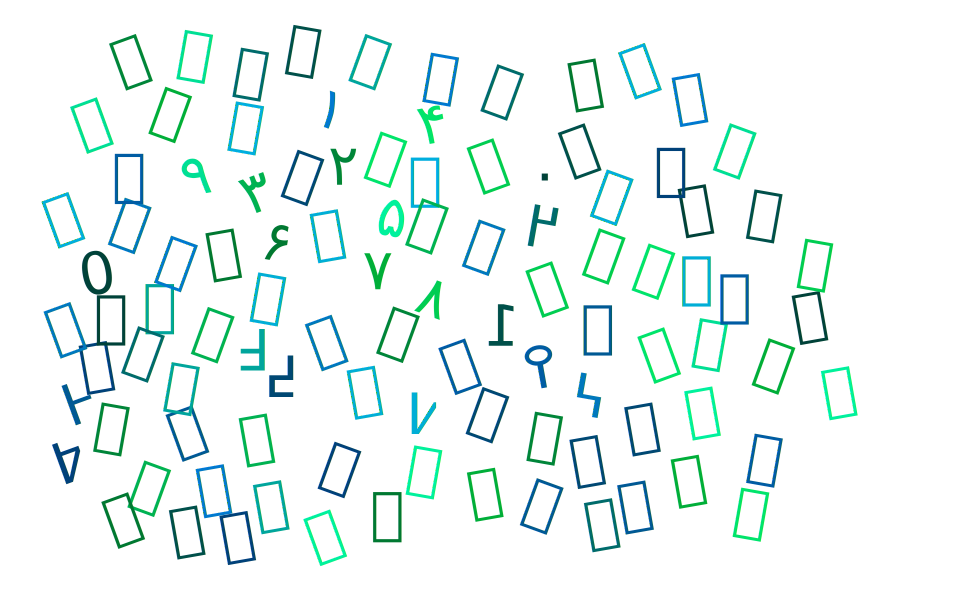
\includegraphics[width=\textwidth]{letternumerals}
  \visible<2->{%
    \begin{tikzpicture}[remember picture,overlay]%
      \node[draw=none,fill=white,font=\Huge,inner sep=5mm,rounded corners=10mm] at (current page.center) {Numerals!};%
    \end{tikzpicture}%
  }
\end{frame}

\begin{frame}
  \frametitle{Character Support}
  \framesubtitle{Numeral Transformation}
  \begin{itemize}
    \item{} \textbf{xmljson} transforms Unicode numerals into their ASCII equivalents
    \item{} \dots{}but only those on the Unicode BMP plane (U+000000 to U+00FFFF)
      \begingroup
      \tiny
  \begin{columns}
    \begin{column}{0.5\textwidth}
      \begin{center}
      \begin{tabular}{lrr}
\texttt{ARABIC-INDIC DIGITS} & \texttt{U+0669} & \texttt{U+0660}\\
\texttt{EXTENDED ARABIC-INDIC DIGITS} & \texttt{U+06F9} &  \texttt{U+06F0}\\
\texttt{NKO DIGITS} & \texttt{U+07C9} &  \texttt{U+07C0}\\
\texttt{DEVANAGARI DIGITS} & \texttt{U+096F} &  \texttt{U+0966}\\
\texttt{BENGALI DIGITS} & \texttt{U+09EF} &  \texttt{U+09E6}\\
\texttt{GURMUKHI DIGITS} & \texttt{U+0A6F} &  \texttt{U+0A66}\\
\texttt{GUJARATI DIGITS} & \texttt{U+0AEF} &  \texttt{U+0AE6}\\
\texttt{ORIYA DIGITS} & \texttt{U+0B6F} &  \texttt{U+0B66}\\
\texttt{TAMIL DIGITS} & \texttt{U+0BEF} &  \texttt{U+0BE6}\\
\texttt{TELUGU DIGITS} & \texttt{U+0C6F} &  \texttt{U+0C66}\\
\texttt{KANNADA DIGITS} & \texttt{U+0CEF} &  \texttt{U+0CE6}\\
\texttt{MALAYALAM DIGITS} & \texttt{U+0D6F} &  \texttt{U+0D66}\\
\texttt{SINHALA LITH DIGITS} & \texttt{U+0DEF} &  \texttt{U+0DE6}\\
\texttt{THAI DIGITS} & \texttt{U+0E59} &  \texttt{U+0E50}\\
\texttt{LAO DIGITS} & \texttt{U+0ED9} &  \texttt{U+0ED0}\\
\texttt{TIBETAN DIGITS} & \texttt{U+0F29} &  \texttt{U+0F20}\\
\texttt{MYANMAR DIGITS} & \texttt{U+1049} &  \texttt{U+1040}\\
\texttt{MYANMAR SHAN DIGITS} & \texttt{U+1099} &  \texttt{U+1090}\\
    \end{tabular}
      \end{center}
    \end{column}
    \begin{column}{0.5\textwidth}
      \begin{center}
      \begin{tabular}{lrr}
\texttt{KHMER DIGITS} & \texttt{U+17E9} &  \texttt{U+17E0}\\
\texttt{MONGOLIAN DIGITS} & \texttt{U+1819} &  \texttt{U+1810}\\
\texttt{LIMBU DIGITS} & \texttt{U+194F} &  \texttt{U+1946}\\
\texttt{NEW TAI LUE DIGITS} & \texttt{U+19D9} &  \texttt{U+19D0}\\
\texttt{TAI THAM HORA DIGITS} & \texttt{U+1A89} &  \texttt{U+1A80}\\
\texttt{TAI THAM THAM DIGITS} & \texttt{U+1A99} &  \texttt{U+1A90}\\
\texttt{BALINESE DIGITS} & \texttt{U+1B59} &  \texttt{U+1B50}\\
\texttt{SUNDANESE DIGITS} & \texttt{U+1BB9} &  \texttt{U+1BB0}\\
\texttt{LEPCHA DIGITS} & \texttt{U+1C49} &  \texttt{U+1C40}\\
\texttt{OL CHIKI DIGITS} & \texttt{U+1C59} &  \texttt{U+1C50}\\
\texttt{VAI DIGITS} & \texttt{U+A629} &  \texttt{U+A620}\\
\texttt{SAURASHTRA DIGITS} & \texttt{U+A8D9} &  \texttt{U+A8D0}\\
\texttt{KAYAH LI DIGITS} & \texttt{U+A909} &  \texttt{U+A900}\\
\texttt{JAVANESE DIGITS} & \texttt{U+A9D9} &  \texttt{U+A9D0}\\
\texttt{MYANMAR TAI LAING DIGITS} & \texttt{U+A9F9} &  \texttt{U+A9F0}\\
\texttt{CHAM DIGITS} & \texttt{U+AA59} &  \texttt{U+AA50}\\
\texttt{MEETEI MAYEK DIGITS} & \texttt{U+ABF9} &  \texttt{U+ABF0}\\
\texttt{FULLWIDTH DIGITS} & \texttt{U+FF19} &  \texttt{U+FF10}\\
    \end{tabular}
      \end{center}
    \end{column}
    \end{columns}
      \endgroup
  \end{itemize}
\end{frame}

\begingroup
  \setbeamercolor{background canvas}{bg=white}
  \begin{frame}[fragile]
    \vspace{-1.15cm}
    \begin{center}
      \includestandalone[width=0.8\textwidth]{resulttable-chars-a}
    \end{center}
  \end{frame}
\endgroup

\begingroup
  \setbeamercolor{background canvas}{bg=white}
  \begin{frame}[fragile]
    \vspace{-1.15cm}
    \begin{center}
      \includestandalone[width=0.8\textwidth]{resulttable-chars-b}
    \end{center}
  \end{frame}
\endgroup

\subsection{Complex XML Documents}

\begingroup
  \setbeamercolor{background canvas}{bg=white}
  \begin{frame}[fragile]
    \vspace{-1.15cm}
    \begin{center}
      \includestandalone[width=0.8\textwidth]{resulttable-complex}
    \end{center}
  \end{frame}
\endgroup

\subsection{Security}

\begin{frame}
  \frametitle{Security}
  \framesubtitle{}
  \begin{itemize}
    \item{} Json-lib is vulnerable to more than 50\% of the attacks tested (DoS, FSA, SSRF)
    \item{} Pesterfish, xmljson and are vulnerable to DoS attacks
      \begin{itemize}
        \item{} Python converters (Pesterfish, xmljson) are insecure if \texttt{ElementTree} parser from the standard
          library is used
        \item{} Alternative: Use hardened \texttt{defusedxml} libary
      \end{itemize}
    \item{} Json.NET is vulnerable for SSRF attacks
  \end{itemize}
\end{frame}

\begingroup
  \setbeamercolor{background canvas}{bg=white}
  \begin{frame}[fragile]
    \vspace{-1.15cm}
    \begin{center}
      \includestandalone[width=0.8\textwidth]{resulttable-sec}
    \end{center}
  \end{frame}
\endgroup

\section{Lossless and secure conversion}

\begin{frame}[fragile]
  \frametitle{JsonML}
  \framesubtitle{JSON Markup Language}
  \begin{itemize}
    \item{} Originally written in JavaScript, but there are also other implementations (e.g. Java: \texttt{org.json.JSONML})
    \item{} Fairly mature: Github repo dates back to November 2006
    \item{} Nicely documented grammar (Backus-Naur form)
    \item{} Downsides:
      \begin{itemize}
        \item{} Resulting \emph{JSON} is not really \enquote{friendly}
        \item{} No support for XML Processing Instructions (no tested solution supports them)
      \end{itemize}
  \end{itemize}
\end{frame}

\begin{frame}[fragile]
  \frametitle{JsonML}
  \framesubtitle{Syntax}
  \begin{center}
    \includestandalone[width=\textwidth]{syntax_jsonml}
  \end{center}
\end{frame}

\begin{frame}[fragile]
  \frametitle{JsonML}
  \framesubtitle{Example}
  \begin{columns}[t]
    \begin{column}{0.45\textwidth}
      \inputminted[breaklines,autogobble,fontsize=\tiny]{xml}{thesis/xmltree.xml}
    \end{column}
    \begin{column}{0.55\textwidth}
      \begin{minted}[breaklines,autogobble,fontsize=\tiny,stripnl=false]{json}



        [ "albums", "\n  ",
          [ "album", { "catno": "ARGO LP-628" }, "\n    ",
            [ "artist", "Ahmad Jamal Trio" ], "\n    ",
            [ "title", "At The Pershing" ], "\n    ",
            [ "recording", "Recorded ", [ "date", "January 16, 1958" ], "." ], "\n  "
          ], "\n"
        ]
      \end{minted}
    \end{column}
  \end{columns}
\end{frame}

\begin{frame}
  \frametitle{JsonML + Processing Instructions}
  \framesubtitle{Adding Support}
  \begin{itemize}
    \item{} JsonML is missing support for Processing Instructions (PIs)
    \item{} Example PI: \mintinline{xml}{<?my-target plus some data?>}
    \item{} Can be described via tuple $P \coloneqq \langle target, data \rangle$
    \item{} JSON representation: \mintinline{json}{["?my-target", "plus some data"]}
    \item{} Tag names may not start with \enquote{\texttt{?}}, so it can't be
      mistaken for an element containing text node
    \item{} If PIs appear outside root element as top level constructs -- Use
      an empty string as parent tag name
  \end{itemize}
\end{frame}

\begin{frame}[fragile]
  \frametitle{JsonML + Processing Instructions}
  \framesubtitle{Syntax Extension}
  \begin{center}
    \includestandalone[width=\textwidth]{syntax_jsonmlpi}
  \end{center}
\end{frame}

\begin{frame}[fragile]
  \frametitle{JsonML + Processing Instructions}
  \framesubtitle{Example}
  \begin{columns}[t]
    \begin{column}{0.45\textwidth}
      \inputminted[breaklines,autogobble,fontsize=\tiny]{xml}{thesis/xmltree.xml}
    \end{column}
    \begin{column}{0.55\textwidth}
      \begin{minted}[breaklines,autogobble,fontsize=\tiny,stripnl=false]{json}
        ["", "\n",
          [ "?xml-stylesheet", "href=\"style.css\"" ],"\n","\n",

          [ "albums", "\n  ",
            [ "album", { "catno": "ARGO LP-628" }, "\n    ",
              [ "artist", "Ahmad Jamal Trio" ], "\n    ",
              [ "title", "At The Pershing" ], "\n    ",
              [ "recording", "Recorded ", [ "date", "January 16, 1958" ], "." ], "\n  "
            ], "\n"
          ]
        ]
      \end{minted}
    \end{column}
  \end{columns}
\end{frame}

\section{Conclusions}

\begin{frame}
  \frametitle{Conclusions}
  \begin{itemize}
    \item{} Converting XML to JSON is not trivial
    \item{} No converter could fully fullfill all requirements out of the box
    \item{} JsonML with added PI support can convert XML in a secure and
      lossless manner
  \end{itemize}
\end{frame}

\begin{frame}
  \frametitle{Limitations}
  \begin{itemize}
    \item{} Focus on XML$\rightarrow$JSON$\rightarrow$XML conversion
    \item{} Parsing DTDs, Entities and Schemas were out of scope
    \item{} Only bi-directional converters (i.e. those that implement inverse
      conversion, too) could be tested
  \end{itemize}
\end{frame}

\begin{frame}
  \frametitle{Future Research}
  \begin{itemize}
    \item{} Look at conversion that uses additional DTD/Schema information
    \begin{itemize}
      \item{} Improve usage of native JSON types
      \item{} Ability to collapse or replace insignificant whitespace
      \item{} Use arrays/objects depending on Schema's \texttt{maxOccurs}
    \end{itemize}
  \item{} Evaluate JSON$\rightarrow$XML$\rightarrow$JSON converters and their
    security
  \item{} Newer technologies like JSON Schema, JSON Include, etc. will probably
    increase attack surface of JSON parsers
    \begin{itemize}
      \item[$\Rightarrow$] closer look might be worthwhile
    \end{itemize}
  \end{itemize}
\end{frame}

%%% Finally the last slide

\begin{frame}[plain]
\frametitle{Thanks!}
  \begin{center}
    {\bfseries\fontsize{30pt}{1.2em}\selectfont Questions?}
  \end{center}
  \begin{columns}
    \begin{column}{0.5\textwidth}
      \begin{center}
        \vbox to 0.54\textheight {
        %\font\endfont = cmss10 at 25.40mm
        %\color{Brown}
        %\endfont
        %\baselineskip 20.0mm
        Reach out via email:
        \begin{itemize}
        \item \textbf{Jan Holthuis}\\
              jan.holthuis@rub.de
        \end{itemize}
        \vfill{}
        {\tiny Title image: Bob Mical, \emph{\enquote{Data Center}} (flickr.com, CC
        BY-NC 2.0)}
      }
      \end{center}
    \end{column}
    \begin{column}{0.5\textwidth}
      \begin{center}
        \pgfimage[width=0.95\textwidth]{questions.jpg}
      \end{center}
    \end{column}
  \end{columns}
\end{frame}

\end{document}
